\documentclass[10pt,letterpaper,twocolumn]{article}

\usepackage[T1]{fontenc}
\usepackage{lmodern}
\usepackage[margin=0.65in,columnsep=0.28in]{geometry}
\usepackage{amsmath,amssymb,mathtools}
\usepackage{graphicx}
\usepackage{xcolor}
\usepackage{microtype}
\usepackage{fancyhdr}
\usepackage{needspace}

\graphicspath{{figures/}}

% The user-local tools/array package is newer than the available LaTeX kernel.
\makeatletter
\def\vcenter@text{\vbox}
\makeatother

\definecolor{navy}{HTML}{17365D}

\pagestyle{fancy}
\fancyhf{}
\fancyhead[L]{\footnotesize Holstein-dimer correction supplement}
\fancyhead[R]{\footnotesize Minimum-norm solver and sensitivity}
\fancyfoot[C]{\thepage}
\renewcommand{\headrulewidth}{0.3pt}

\setlength{\parindent}{0pt}
\setlength{\parskip}{3.2pt plus 0.5pt}
\setlength{\abovedisplayskip}{6pt plus 2pt minus 2pt}
\setlength{\belowdisplayskip}{6pt plus 2pt minus 2pt}
\setlength{\abovedisplayshortskip}{4pt plus 1pt}
\setlength{\belowdisplayshortskip}{4pt plus 1pt}
\newcommand{\R}{\mathbb R}
\newcommand{\C}{\mathbb C}
\newcommand{\ii}{\mathrm i}
\newcommand{\sectionline}[1]{%
  \Needspace{6\baselineskip}%
  \par\medskip{\color{navy}\large\bfseries #1}\par
  \vspace{-2pt}{\color{navy}\rule{\columnwidth}{0.7pt}}\par\smallskip
}

\begin{document}
\raggedbottom

\twocolumn[
\begin{center}
  {\color{navy}\LARGE\bfseries Minimum-Norm Physicality Correction}\par\vspace{3pt}
  {\large Standalone derivation and controller-sensitivity diagnostics}\par
\end{center}
\vspace{2pt}\hrule\vspace{6pt}
]

\sectionline{1. From the raw velocity to structured matrix changes}

At one right-hand-side evaluation, the retained state is
\(X=(\rho,B,N,A,C)\), represented by a real coordinate vector
\(x\in\R^{31}\).  The archive equations evaluate the instantaneous
coordinate velocity
\[
\dot x_0=f(t,x).
\tag{S.1}
\]
The controller chooses a real correction \(w\in\R^{31}\), whose entries are
\(w=(w_0,\ldots,w_{30})\).  It supplies the integrator with
\[
\dot x_{\rm c}=\dot x_0+w.
\tag{S.2}
\]
The current state \(x\) is held fixed during this solve.  The quantity being
selected is its velocity for the present Runge--Kutta evaluation.

The entries of \(w\) follow the same ordering as the entries of \(x\).  Their
\emph{structured lift} places the independent real coefficients into matrix
velocities.  The electronic and phononic parts are
{\footnotesize
\[
\begin{aligned}
\Delta\dot\rho(w)&=
\begin{pmatrix}
w_0/2&w_1+\ii w_2\\
w_1-\ii w_2&-w_0/2
\end{pmatrix},\\
\Delta\dot B(w)&=
\begin{pmatrix}w_3+\ii w_4\\w_5+\ii w_6\end{pmatrix},\\
\Delta\dot N(w)&=
\begin{pmatrix}
w_7&w_9+\ii w_{10}\\
w_9-\ii w_{10}&w_8
\end{pmatrix},\\
\Delta\dot A(w)&=
\begin{pmatrix}
w_{11}+\ii w_{12}&w_{15}+\ii w_{16}\\
w_{15}+\ii w_{16}&w_{13}+\ii w_{14}
\end{pmatrix}.
\end{aligned}
\tag{S.3}
\]
}
The lift preserves the trace of \(\rho\), Hermiticity of \(\rho\) and
\(N\), and symmetry of \(A\).  The two correlation matrices receive
{\scriptsize
\[
\begin{aligned}
\Delta\dot C^0(w)&=
\begin{pmatrix}
\frac{w_{17}+\ii w_{18}+w_{19}+\ii w_{20}}2&w_{21}+\ii w_{22}\\
w_{23}+\ii w_{24}&\frac{w_{17}+\ii w_{18}-w_{19}-\ii w_{20}}2
\end{pmatrix},\\[2pt]
\Delta\dot C^1(w)&=
\begin{pmatrix}
\frac{w_{17}+\ii w_{18}+w_{25}+\ii w_{26}}2&w_{27}+\ii w_{28}\\
w_{29}+\ii w_{30}&\frac{w_{17}+\ii w_{18}-w_{25}-\ii w_{26}}2
\end{pmatrix}.
\end{aligned}
\tag{S.4}
\]
}
The shared entries \(w_{17}+\ii w_{18}\) change
\(\operatorname{Tr}C^0\) and \(\operatorname{Tr}C^1\) by the same amount.

The physicality test uses the electronic density and the joint Gram matrix
\[
\mathcal G=
\begin{pmatrix}
M_{\rm B}(N,A)&Z(C)\\
Z(C)^\dagger&E(\rho)
\end{pmatrix},
\tag{S.5a}
\]
\[
M_{\rm B}(N,A)=
\begin{pmatrix}
N^{\mathsf T}&A^*\\
A&I_2+N
\end{pmatrix}.
\tag{S.5b}
\]
Differentiating these block constructions along (S.3)--(S.4) produces the
Hermitian matrix change \(\Delta\dot{\mathcal G}(w)\).  This is the first
important map:
\[
w\in\R^{31}
\ \longmapsto\
\bigl(\Delta\dot\rho(w),\Delta\dot{\mathcal G}(w)\bigr).
\tag{S.6}
\]
One scalar entry of \(w\) may appear in several matrix entries because the
lift retains the matrix symmetries.

For a scalar eigenvalue margin \(m(t)\), the differential barrier condition
is
\[
\dot m+\beta(m-h_\star)\geq0,
\tag{S.7}
\]
where \(h_\star>0\) is the desired interior margin and \(\beta>0\) sets its
recovery rate.  Multiplication by \(e^{\beta t}\) and integration give
\[
m(t)\geq h_\star+[m(0)-h_\star]e^{-\beta t}.
\tag{S.8}
\]
At the boundary \(m=h_\star\), the allowed velocity satisfies
\(\dot m\geq0\).  The matrix form applies this condition to every eigenvalue
direction.  At the fixed state \(x\), the three corrected barrier matrices
are
{\footnotesize
\[
\begin{aligned}
M_{\rho^-}(w)
&=\dot\rho_0+\Delta\dot\rho(w)
  +\beta(\rho-h_\star I_2),\\
M_{\rho^+}(w)
&=-\dot\rho_0-\Delta\dot\rho(w)
  +\beta(I_2-\rho-h_\star I_2),\\
M_{\mathcal G}(w)
&=\dot{\mathcal G}_0+\Delta\dot{\mathcal G}(w)
  +\beta(\mathcal G-h_\star I_7).
\end{aligned}
\tag{S.9}
\]
}
They enforce the lower electronic boundary \(\rho\succeq0\), the upper
electronic boundary \(I_2-\rho\succeq0\), and joint-Gram positive
semidefiniteness.

The correction also preserves the correlation trace and contributes zero
instantaneous internal-energy flux.  With
\(s=\operatorname{Tr}C^q=x_{17}+\ii x_{18}\), these three scalar equations
are
\[
\begin{aligned}
\dot x_{0,17}+w_{17}+\beta x_{17}&=0,\\
\dot x_{0,18}+w_{18}+\beta x_{18}&=0,\\
\nabla_xE_{\rm int}(x)^{\mathsf T}w&=0.
\end{aligned}
\tag{S.10}
\]
The complete controller therefore seeks the shortest \(w\) satisfying
(S.9)--(S.10).

\sectionline{2. Continuous derivation of the minimum correction}

Write the three scalar equations as one linear system
\[
Lw=d,
\tag{S.11}
\]
where \(L:\R^{31}\to\R^3\) is defined by
\[
Lw=
\begin{pmatrix}
\nabla_xE_{\rm int}(x)^{\mathsf T}w\\
w_{17}\\
w_{18}
\end{pmatrix},
\qquad
d=
\begin{pmatrix}
0\\
-\dot x_{0,17}-\beta x_{17}\\
-\dot x_{0,18}-\beta x_{18}
\end{pmatrix}.
\tag{S.12}
\]
The first task is to identify which directions in the 31-dimensional
correction space change these three scalar quantities and which directions
leave them fixed.  Let \(r\) be the rank of \(L\).  Its reduced
singular-value decomposition is
\[
L=U\Sigma V^{\mathsf T},
\tag{S.13}
\]
with \(U\in\R^{3\times r}\),
\(\Sigma\in\R^{r\times r}\), and
\(V\in\R^{31\times r}\).  The columns of \(U\) and \(V\) are orthonormal,
and the diagonal entries of \(\Sigma\) are positive.

The multiplication in (S.13) is a sequence of three maps:
\[
w
\ \longmapsto\ V^{\mathsf T}w
\ \longmapsto\ \Sigma V^{\mathsf T}w
\ \longmapsto\ U\Sigma V^{\mathsf T}w=Lw.
\tag{S.14}
\]
The first map reads the components of \(w\) along the directions that affect
the equalities.  The second scales each component by the strength with which
it affects them.  The third combines those scaled components into the energy
condition and the two trace conditions.  Thus the columns of \(V\) span the
equality-changing directions.

Let \(Q\in\R^{31\times(31-r)}\) contain orthonormal columns perpendicular to
the columns of \(V\).  Then
\[
V^{\mathsf T}Q=0,
\qquad Q^{\mathsf T}Q=I_{31-r},
\qquad LQ=0.
\tag{S.15}
\]
The columns of \(Q\) span the equality-preserving directions.  Every
correction can therefore be written uniquely as
\[
w=V\alpha+Qy,
\qquad
\alpha\in\R^r,
\quad y\in\R^{31-r}.
\tag{S.16}
\]
Substituting this form into \(Lw=d\) gives
\[
U\Sigma\alpha=d,
\qquad
\alpha=\Sigma^{-1}U^{\mathsf T}d.
\tag{S.17}
\]
Consequently,
\[
w=w_{\rm p}+Qy,
\qquad
w_{\rm p}=V\Sigma^{-1}U^{\mathsf T}d.
\tag{S.18}
\]
The vector \(w_{\rm p}\) is the shortest correction satisfying the three
scalar equations.  The variable \(y\) now carries every remaining freedom,
and changing \(y\) preserves those equations because \(LQ=0\).  Orthogonality
also gives
\[
\|w\|^2=\|w_{\rm p}\|^2+\|y\|^2.
\tag{S.19}
\]
The matrix constraints can therefore select the shortest admissible \(y\).

Choose any one of the three barrier matrices in (S.9) and denote it by
\[
M(w)=M_0+\Delta M(w)\in\C_{\rm H}^{m\times m},
\qquad m\in\{2,7\}.
\tag{S.20}
\]
Here \(M_0=M(0)\) is the barrier produced by the raw velocity, and
\(\Delta M(w)\) is the structured matrix change induced by the correction.
At cutting-plane iteration \(k\), set
\(w^{(k)}=w_{\rm p}+Qy^{(k)}\), diagonalize \(M(w^{(k)})\), and take its
smallest eigenpair:
\[
\begin{aligned}
M(w^{(k)})v&=\lambda v,\\
v^\dagger v&=1,\\
\lambda&=\lambda_{\min}(M(w^{(k)}))<0.
\end{aligned}
\tag{S.21}
\]
The normalized vector \(v=(v_1,\ldots,v_m)^{\mathsf T}\) gives the
coefficients of the particular barrier-space direction with the smallest
margin.  Its dimension is \(m\).  The correction \(w\) has dimension 31 and
acts on that barrier direction through the lift.  The quadratic form evaluates
the scalar margin along \(v\):
\[
v^\dagger M(w^{(k)})v
=v^\dagger(\lambda v)
=\lambda.
\tag{S.22}
\]

We now need the sensitivity of this scalar margin to each coordinate of
\(w\).  At this exact step, define the 31-dimensional unit vector
\[
e_j=(0,\ldots,0,\underbrace{1}_{j\text{th position}},0,\ldots,0)^{\mathsf T}.
\tag{S.23}
\]
The vector \(e_j\) activates one coordinate of the correction.  Its lift
\(\Delta M(e_j)\) is the complete Hermitian matrix pattern produced by one
unit of \(w_j\).  The scalar
\[
a_j=v^\dagger\Delta M(e_j)v
=\sum_{r=1}^{m}\sum_{s=1}^{m}
v_r^*[\Delta M(e_j)]_{rs}v_s
\tag{S.24}
\]
is therefore the change of the exposed barrier margin per unit of coordinate
\(w_j\).  Hermiticity makes \(a_j\) real.  Collect these sensitivities into
\(a=(a_0,\ldots,a_{30})^{\mathsf T}\in\R^{31}\).

Since the lift is linear,
\[
\Delta M(w-w^{(k)})
=\sum_{j=0}^{30}(w_j-w_j^{(k)})\Delta M(e_j).
\tag{S.25}
\]
Contracting this identity with \(v\) produces the exact affine relation
\[
\begin{aligned}
v^\dagger M(w)v
&=\lambda+
  \sum_{j=0}^{30}a_j(w_j-w_j^{(k)})\\
&=\lambda+a^{\mathsf T}(w-w^{(k)}).
\end{aligned}
\tag{S.26}
\]
The correction changes the matrix through its lifted entry patterns, and the
matrix change raises the scalar value along the failing direction.  Requiring
that value to reach the PSD boundary gives
\[
a^{\mathsf T}w
\geq a^{\mathsf T}w^{(k)}-\lambda.
\tag{S.27}
\]
This inequality is a half-space in the 31 correction coordinates.  Its normal
vector \(a\) points in the coordinate-space direction that raises the exposed
margin most efficiently per unit Euclidean displacement.

Substitute the equality-preserving form
\(w=w_{\rm p}+Qy\) into (S.27).  With
\[
n=Q^{\mathsf T}a,
\qquad
c=n^{\mathsf T}y^{(k)}-\lambda,
\tag{S.28}
\]
the cut becomes \(n^{\mathsf T}y\geq c\).  The one-cut problem is now
\[
\begin{aligned}
y^\star\in\underset{y\in\R^{31-r}}{\operatorname{argmin}}\quad
&\frac12y^{\mathsf T}y\\
\text{subject to}\quad&n^{\mathsf T}y\geq c.
\end{aligned}
\tag{S.29}
\]
For \(c>0\), introduce the nonnegative Lagrange multiplier \(\mu\) and write
\[
\mathcal L(y,\mu)
=\tfrac12y^{\mathsf T}y-\mu(n^{\mathsf T}y-c).
\tag{S.30}
\]
Stationarity and the active boundary give
\[
y-\mu n=0,
\qquad n^{\mathsf T}y=c.
\tag{S.31}
\]
Solving these equations yields
\[
y^\star=\frac{c}{\|n\|^2}n,
\qquad
w^\star=w_{\rm p}+Qy^\star.
\tag{S.32}
\]
For \(c\leq0\), \(y=0\) already belongs to the half-space and has the
smallest norm.  Equation (S.32) therefore adds exactly the shortest
equality-preserving displacement needed to reach the exposed matrix boundary.

The geometric core is clearest when the scalar equality rows are temporarily
removed.  Then \(Q=I_{31}\), \(w_{\rm p}=0\), the first cut is evaluated at
\(w^{(0)}=0\), and \(c=-\lambda\).  Equation (S.32) reduces to
\[
\boxed{
w^\star=-\frac{\lambda}{\|a\|^2}a
}
\tag{S.33}
\]
and direct substitution gives
\[
v^\dagger M(w^\star)v
=\lambda+a^{\mathsf T}w^\star
=\lambda-\lambda=0.
\tag{S.34}
\]
The negative amount \(\lambda\) is cancelled by the induced matrix response
\(v^\dagger\Delta M(w^\star)v=-\lambda\).  The controller changes \(M\) by
combining the allowable Hermitian patterns \(\Delta M(e_j)\); the eigenvalue
responds to that matrix change.

One eigenvector supplies one half-space.  Complete positive semidefiniteness
requires
\[
\begin{aligned}
M(w)\succeq0
\quad\Longleftrightarrow\quad
&\xi^\dagger M(w)\xi\geq0\\
&\text{for every normalized }\xi.
\end{aligned}
\tag{S.35}
\]
After solving the current half-space problem, the implementation rebuilds and
diagonalizes all three barrier matrices.  A newly exposed negative eigenvector
supplies another cut.  With accumulated cuts
\(n_i^{\mathsf T}y\geq c_i\), the actual reduced solve is
\[
\begin{aligned}
\underset{y\in\R^{31-r}}{\operatorname{minimize}}\quad
&\tfrac12\|y\|^2\\
\text{subject to}\quad
&n_i^{\mathsf T}y\geq c_i,
\qquad i=1,\ldots,p.
\end{aligned}
\tag{S.36}
\]
The Sequential Least Squares Programming (SLSQP) numerical optimizer computes
the shortest point in this intersection.  The cycle ends when
the lower electronic, upper electronic, and joint-Gram barrier matrices all
meet the eigenvalue tolerance.  The resulting \(w^\star\) is added to the raw
velocity at the current Runge--Kutta evaluation.

\sectionline{3. What the controller-sensitivity diagnostics measure}

The derivation above contains three linked objects.  The eigenvector \(v\)
identifies the weakest direction in a barrier matrix.  The coordinate
sensitivities \(a_j=v^\dagger\Delta M(e_j)v\) measure how strongly each
allowed velocity coordinate changes that direction.  The optimized
correction \(w^\star\) combines those coordinates while satisfying every
active cut together with the energy and trace equations.

To isolate the portion inserted by joint-Gram positive semidefiniteness, let
\(w_{\rm e}(t)\) be the minimum-norm correction satisfying only the energy and
trace equations, and define
\[
w_{\rm g}(t)=w^\star(t)-w_{\rm e}(t).
\tag{S.37}
\]
For each retained block \(Y\in\{\rho,B,N,A,C\}\), let
\(w_{{\rm g},Y}\) denote the entries of \(w_{\rm g}\) belonging to that
block.  Its integrated share of the joint-cone action is
\[
\eta_Y=
\frac{\displaystyle\int_0^T\|w_{{\rm g},Y}(t)\|^2\,dt}
     {\displaystyle\int_0^T\|w_{\rm g}(t)\|^2\,dt}.
\tag{S.38}
\]
The measured shares were
\[
(\eta_\rho,\eta_B,\eta_N,\eta_A,\eta_C)
=(23.37,\ 2.14,\ 0.80,\ 4.52,\ 69.18)\%.
\tag{S.39}
\]
Thus the optimization supplied most of its additional cone-preserving
velocity through the electron--phonon correlation coordinates, followed by
the electronic-density coordinates.

The lower diagnostic resolves the weakest normalized eigenvector of the
\(7\times7\) joint Gram matrix.  Its squared norm averaged over the same
cone-action weighting was \(62.97\%\) in the three electronic Pauli
directions and \(37.03\%\) in the four bosonic directions.  The largest
individual weights were \(34.11\%\) in \(\delta\sigma_z\), \(24.51\%\) in
\(\delta\sigma_y\), and \(30.24\%\) in the two phonon-annihilation entries
together.  The exposed barrier is therefore a mixed electron--phonon mode,
while its optimized repair is carried primarily by the correlation and
electronic-density velocity coordinates.

\begin{center}
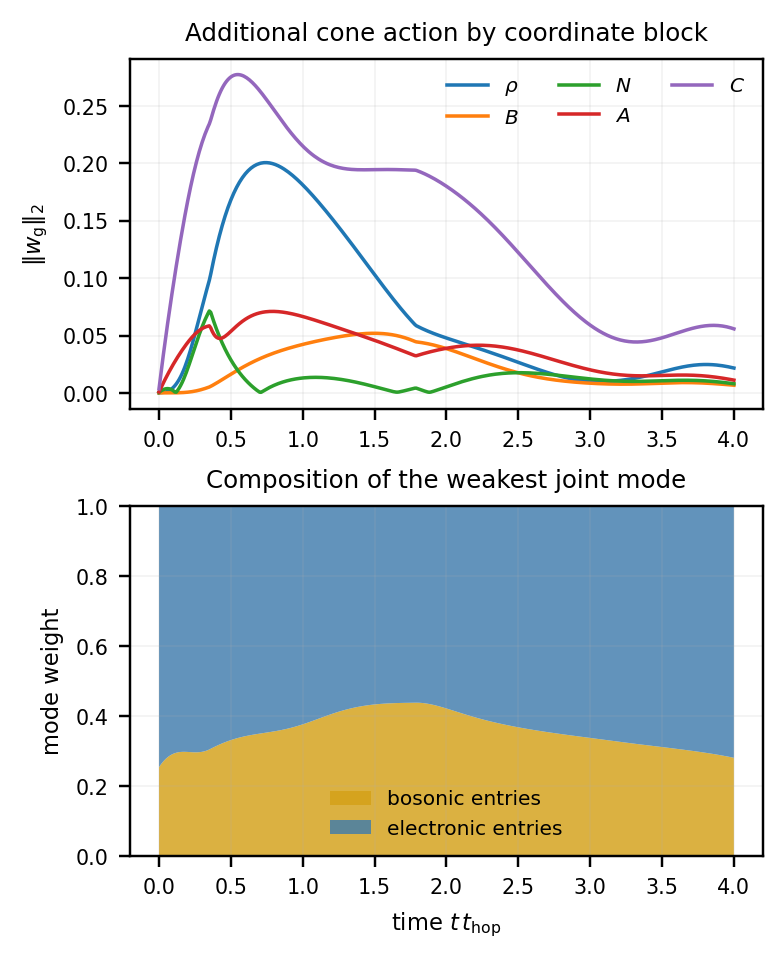
\includegraphics[width=0.83\columnwidth]{joint_electron_phonon_mechanism_evidence.pdf}

\parbox{0.94\columnwidth}{\small
\textbf{Controller-sensitivity diagnostic.}
The upper panel measures where the optimized joint-cone correction
\(w_{\rm g}\) is placed in the 31-coordinate velocity.  The lower panel
measures the bosonic and electronic composition of the weakest joint-Gram
direction \(v\).}
\end{center}

\end{document}
